% % % % % % % % % % % % % % % % % % % % % % % % % % % % % % % % % % % %
\documentclass[english]{article}
\usepackage[T1]{fontenc}
\usepackage[latin9]{inputenc}
\usepackage{fancyhdr}
\pagestyle{fancy}
\usepackage{textcomp}
\usepackage{babel}
\usepackage{url}
\usepackage{color,soul}
\usepackage{graphicx}
\usepackage[pdftitle={Adaptive Geo--Replication Based on Ant Colony Algorithm},%
		hidelinks,colorlinks=true, linkcolor=black, citecolor=cyan, filecolor=green, urlcolor=blue]{hyperref}
\usepackage{mathtools}
\usepackage{amssymb}
\usepackage[numbers]{natbib}
%\usepackage{glossaries}
%\usepackage[xindy]{glossaries}

\usepackage{multirow}
\usepackage{rotating}

\graphicspath{{./figures/}}


\definecolor{msgTxt}{RGB}{51,51,178}

%\makeglossaries

% % % % % % % % % % % % % % % % % % % % % % % % % %
% Aconyms for SyncFree project.
%
% Author: Amadeo Asco 
% Last updated: 24 July 2014
% % % % % % % % % % % % % % % % % % % % % % % % % %
% The acronym package helps you manage acronyms and acronym lists in your documents, http://www.mackichan.com/index.html?techtalk/456.htm~mainFrame
% for the glossary to show up in Table of Contents you need to additionally add toc option
\usepackage[toc,nonumberlist]{glossaries}
%\showthe\hsize% interrupts latex and shows value of \hsize
\setlength{\glsdescwidth}{0.82\hsize}%
% to remove extra line between groups
\renewcommand{\glsgroupskip}{}
% To get rid of the full stop after the description in the glossary
\renewcommand{\glspostdescription}{}
\makeglossaries

% Start definitions ---------------------------
% Add all of the definitions for the abbreviations
\newacronym{2pc}{2PC}{two-phase commit}
\newacronym{2i}{2i}{Secondary Indexing}
\newacronym{2pset}{2P-Set}{Two-Phase Set}
\newacronym{acid}{ACID}{Atomicity, Consistency, Isolation, Durability}
\newacronym{api}{API}{Application Programming Interface}
\newacronym{b2b}{B2B}{Business to Business}
\newacronym{base}{BASE}{basically available, soft state, eventual consistency}
\newacronym{cci}{CCI}{Causality, Convergence and Intention}
\newacronym{cmrdt}{CmRDT}{Op-based Convergent Replicated Data Type}
\newacronym{cprdt}{CPRDT}{Conflict-free Partially Replicated Data Type}
\newacronym{crdt}{CRDT}{Conflict-free Replicated Data Type}
\newacronym{cqrs}{CQRS}{Command Query Responsibility Segregation}
\newacronym{cvrdt}{CvRDT}{State-based Convergent Replicated Data Type}
\newacronym{db}{DB}{Data Base}
\newacronym{dc}{DC}{Data Centre}
\newacronym{ec}{EC}{Eventual Consistency}
\newacronym{fmk}{FMK}{Shared Medical Record}
\newacronym{ga}{GA}{Genetic Algorithm}
\newacronym{gmu}{GMU}{Genuine Multi-version Update}
\newacronym{gp}{GP}{General Practitioner}
\newacronym{gpr}{GPR}{Genuine Partial Replication}
\newacronym{gset}{G-set}{State-based increment-only Counter}
\newacronym{ha}{HA}{High Availability}
\newacronym{id}{ID}{identifier}
\newacronym{iot}{IoT}{Internet of Things}
\newacronym{lww}{LWW}{Last-Writer-Wins}
\newacronym{lwwr}{LWW-Register}{Last-Writer-Wins Register}
\newacronym{mdc}{MDC}{Multi Data Centre}
\newacronym{mv}{MV}{Multi-Valued}
\newacronym{mvr}{MV-Register}{Multi-Valued Register}
\newacronym{orset}{OR-set}{Observed-Removed Set}
\newacronym{pb}{PB}{petabytes}
\newacronym{rdbms}{RDBMS}{Relational Database Management System}
\newacronym{rga}{RGA}{Replicated Growing Array}
\newacronym{rest}{REST}{Representational State Transfer}
\newacronym{rpc}{RPC}{Remote Procedure Call}
\newacronym{cap}{CAP}{Consistency, Availability and Partition tolerance}
\newacronym{sec}{SEC}{Strong Eventual Consistency}
\newacronym{tb}{TB}{terabyte}
\newacronym{ttl}{TTL}{Time To Live}
\newacronym{uset}{U-Set}{Two-Phase Set with unique elements}
\newacronym{wp1}{WP 1}{Work Package 1}
\newacronym{wp2}{WP 2}{Work Package 2}
\newacronym{wp3}{WP 3}{Work Package 3}
\newacronym{wp4}{WP 4}{Work Package 4}
\newacronym{wp5}{WP 5}{Work Package 5}
\newacronym{uml}{UML}{Unified Modelling Language}
% end abbreviations ---------------------------

%\ifnum\showDefinitions=1
% Add all of the definitions
%\newglossaryentry{bwd}{name={box-and-whisker diagram}, text={box-and-whisker diagram}, first={box-and-whisker diagram},
%    description={\parbox{10.6cm}{\medskip The bottom and top of the box are the 25th and 75th percentile (the lower and upper quartiles, respectively), and the band near the middle of the box is the median, whereas the dot represent the mean. The ends of the whiskers represent the minimum and maximum of all of the data.\medskip}}}
% end definitions -----------------------------
%\fi

\glsdisablehyper


\begin{document}

\title{Adaptive Geo--Replication\\Design}

\author{Amadeo Asc\'{o}\\ Trifork Leeds, Leeds, UK}

\date{13$^{th}$ November 2014}

\maketitle

%{\bf Keywords}: Adaptive Replication, SyncFree, design, implementation

\section{Adaptive Replication}
A common technique to reduce latency is the replication of data between different DCs in a system with multiple \glspl{dc} distributed around the world, as shown in Figure \ref{fig:full_replication}. But keeping multiple replicas is an expensive commodity given the increase in storage requirements and bandwidth as a write operation needs to be propagated to all the other \glspl{dc} with a replica. The data could be placed in only one DC, in which case there is not any replication, or a copy could exist in all the available \glspl{dc}, which it is known as full replication. Alternatively the data may be located in some but not necessarily all the \glspl{dc} such that the number, location and data is determined at run time, which it is known as adaptive replication.
\begin{figure}[ht!]
	\centering
	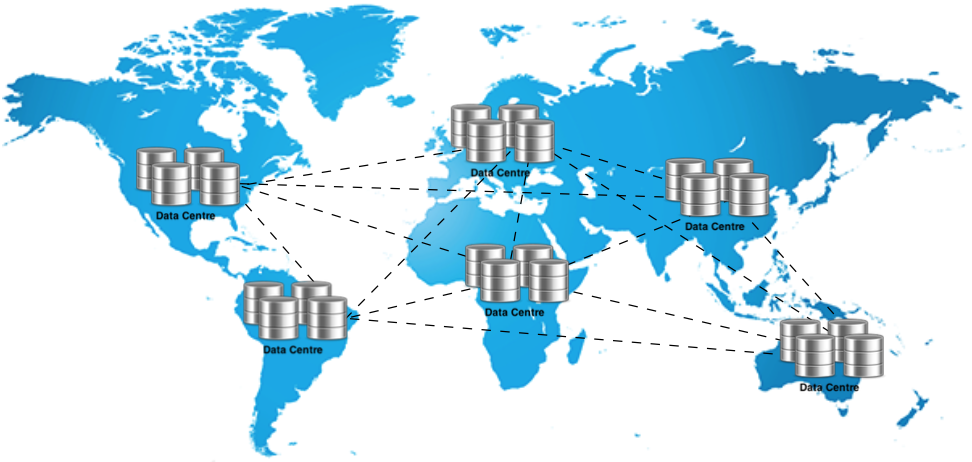
\includegraphics[width=1\textwidth]{multiDCs.png}
	
	\caption{Layers view.}
	\label{fig:full_replication}
\end{figure}

The replications may be grouped, base on its existence, into two types; static replication where a replica persist until it is deleted by a user or its duration expires, and dynamic replication where the creation and deletion of a replica are managed automatically and normally directed by the access pattern of the data used by the users \cite{Dong2008a}. In static replication the major drawback is their inability to adapt to changes in the access pattern of the data used by the users.

Adaptive geo--replication is concerned in what and where the data is located within the overall system of \glspl{dc} and how many replicas exist simultaneously, \cite{Jeon2014a, Ardekani2014a, KingsyGrace2013a, Wang2012a, Abad2011a, Abdul-Wahid2007a, Loukopoulos2004a}. This is also know as \textquotedblleft Adaptive Location of Replicas\textquotedblright. In the example, shown in Figure \ref{fig:adaptive_replication}, data reads/writes to \glspl{dc} 1 and 2 making the data replica to move from \gls{dc} 3 to \glspl{dc} 1 and 2 ensuring that the data is closer to where the reads and writes are requested based on the specified objectives and constraints.
\begin{figure}[ht!]
	\centering
	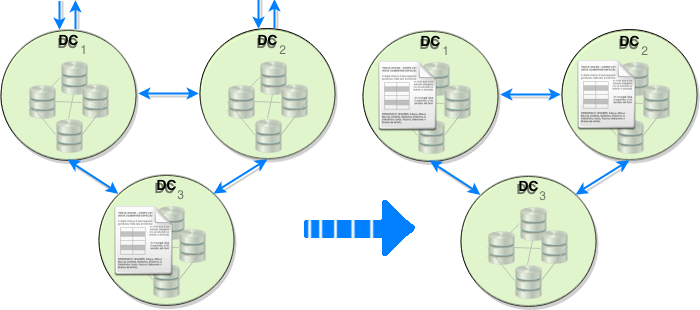
\includegraphics[width=1\textwidth]{adaptiveReplication.png}
	
	\caption{Example of adaptive geo--replication.}
	\label{fig:adaptive_replication}
\end{figure}


\section{Implementation}
Layers required to dissociate both the strategy  and the replication, see Figure \ref{fig:layers_view}. These layers are:
\begin{itemize}
	\item \textquotedblleft{\bf Startegy Layer}\textquotedblright\\
	Responsible to control the replication process.
	
	\item \textquotedblleft{\bf Replication Layer}\textquotedblright\\
	Responsible to maintain the replication, deal with the communication between \glspl{dc} and keep the assurances such as eventual consistency.
\end{itemize}
\begin{figure}[ht!]
	\centering
	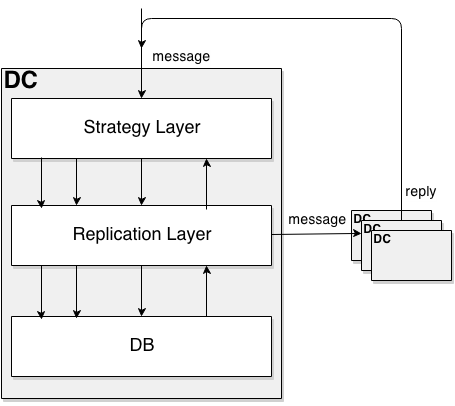
\includegraphics[width=1\textwidth]{adatativeReplicationLayers.png}
	
	\caption{Layers view.}
	\label{fig:layers_view}
\end{figure}

All the messages (operations) are received first by the strategy that may convert them to other messages based on its implementation. Some operations are required:
\begin{itemize}	
	\item {\bf Read}\\
	Request sent by a client to a \gls{dc}. If the data is not replicated then forward it to appropriate \gls{dc}, so here it is where \textquotedblleft Has replica\textquotedblright messages are sent to all other \glspl{dc} to determine the most appropriate \gls{dc} to forward the request, which constitute the discovery state. This may be required to do it once, the first time, and the result may be used in subsequent messages. The \gls{dc} receiving the forward read message will reply with the data, assuming it does still have a replica, otherwise return a read reply with an error code and the the discovery must be executed again.
	
	It must contain at least a message unique ID, the message type, the originator of the message the data key.
	
	\item {\bf Has replica}\\
	Request sent by a \gls{dc} to another \gls{dc}, which will reply only if the destination \gls{dc} has a replica of the data. This could be similar to a read but without the returning any data, so more efficient if the data to return is large.
	
	It must contain at least  a message unique ID, the message type, the originator of the message and the data key.

	\item {\bf Create}\\
	Request sent by a client to a \gls{dc} to create the data. Once the data is created some other operations may be sent by the strategy from the \textquotedblleft Strategy Layer\textquotedblright to fulfil constraints, e.g. minimum number of replicas.
	
	It must contain at least  a message unique ID, the message type, the originator of the message and data tuple key, value.

	\item {\bf Write}\\
	Request sent by a client to a \gls{dc}t to change the value of the data. If the data is not replicated then forward it to appropriate \gls{dc}, so here it is where \textquotedblleft Has replica\textquotedblright messages are sent to all other \glspl{dc} to determine the most appropriate \gls{dc} to forward the request, which constitute the discovery state. This may be required to do it once, the first time, and the result may be used in subsequent messages. The \gls{dc} receiving the forward write message will change the data locally and send update messages to all the other \glspl{dc} with replicas.
	
	It must contain at least  a message unique ID, the message type, the originator of the message and the data tuple key, value.

	\item {\bf Update}\\
	Request sent by a \gls{dc} to another \gls{dc} with a replica, which will update its version of the data, the replica. This message type could by implemented as a type of forward message.

	It must contain at least  a message unique ID, the message type, the originator of the message and the data tuple key, value.

	\item {\bf New replica}\\
	Notification from a \gls{dc} to one or many of the other \glspl{dc} to let the \glspl{dc} know that it has a replica. If the notification is sendt from original \gls{dc} to one of the \glspl{dc} with replicas that the destination \gls{dc} must notify all the other \glspl{dc} with replicas and reply to the originator \gls{dc} with a list of the current \glspl{dc} with replicas.
	
	It must contain at least  a message unique ID, the message type, the originator of the message and the data identifying the new \gls{dc} with a replica.

	\item {\bf Remove replica}\\
	Notification from a \gls{dc} to all the other \glspl{dc} that the \gls{dc} will not have a replica anymore. Here there must be some negotiation between the \glspl{dc} to make sure some of the constraints are guarantee, i.e. minimum number of \glspl{dc}.

	It must contain at least  a message unique ID, the message type, the originator of the message and the data identifying the \gls{dc} with a replica, which coincides with the originator of the message.

	\item {\bf Forward}
		\begin{itemize}
			\item \underline{Read}\\
			Request sent by another \gls{dc} which it is replied with the loca value of the data (it is an standard read).

			\item \underline{Write}\\
			Request sent by another \gls{dc} which changes the local data and sends update messages to all the other \glspl{dc}.
		\end{itemize}

	\item {\bf Reply}
		\begin{itemize}
			\item \underline{Read}\\
			The reply message result from a previous read request containing the read data.

			It must contain at least the original message unique ID, the tuple key, value for the data requested.

			\item \underline{Write}\\
			The reply message result from a previous write request.

			It must contain at least the original message unique ID, and an indication of success.

			\item \underline{Has replica}\\
			The reply message result from a previous \textquotedblleft Has replica\textquotedblright request containing the list of current \glspl{dc} with a replica of the data.

			It must contain at least the original message unique ID, and the original destination \gls{dc} or a list of all the current \glspl{dc} with a replica.

			\item ...
		\end{itemize}
\end{itemize}

All the internal communication could be done by forward messages so requests like \textquotedblleft Update\textquotedblright, \textquotedblleft New replica\textquotedblright, \textquotedblleft Remove replica\textquotedblright and \textquotedblleft Has replica\textquotedblright could be other sub-types of forward messages.

There is also the need to convert replies from other \glspl{dc} to forward requests into replies to original requesters and send them to those requesters.

It is required a way to get information stored in the underlying \textquotedblleft Materializer\textquotedblright, such as the list of current \glspl{dc}.

There is a question about the location of the extra data required by the strategy.\\

\subsection{Messages per layer}
All the messages go through the {\bf Strategy Layer} which may convert them to another or many other messages that are passed to the {\bf Replication Layer}. The messages received and processed by each layer are presented below.

At the {\bf Strategy Layer} level the messages are
\begin{itemize}
	\item From $client$:
		\begin{itemize}
			\item \textcolor{msgTxt}{create}\\
				Create the data for first time. Initially processed in the Strategy Layer and completed in the Replication Layer.
			\item \textcolor{msgTxt}{read}\\
				Read data with specified key. Initially processed in the Strategy Layer and maybe completed in the Replication Layer.
			\item \textcolor{msgTxt}{write}\\
				Write specified tuple key, value. Initially processed in the Strategy Layer and maybe completed in the Replication Layer.
		\end{itemize}

	\item From another  $\gls{dc}$:
		\begin{itemize}
			\item \textcolor{msgTxt}{has\_replica}\\
				It is processed in the $Strategy Layer$. Sending this messages to \glspl{dc} without replica will fail and failure should be ignored, otherwise the \gls{dc} receiving the message replies with the list of \glspl{dc} with replicas, inclusive of itself.
			\item \textcolor{msgTxt}{update}\\
				It implies that a write was done in another \gls{dc}. Processed in the Strategy Layer and pass to $Replication Layer$.
			\item \textcolor{msgTxt}{rmv}\\
				It indicates that the local replica must be removed, and the data process. Passed to Replication Layer.
			\item \textcolor{msgTxt}{new\_replica}\\
				It is received from another \gls{dc} that now has a replica. Passed to Replication Layer.
			\item \textcolor{msgTxt}{rmv\_replica}\\
				It is passed to Replication Layer.
			\item \textcolor{msgTxt}{forward}
				\begin{itemize}
					\item \textcolor{msgTxt}{read}\\
						It is processed in the Strategy Layer but may need the Replication Layer, depends on where it is cashed.
					\item \textcolor{msgTxt}{write}\\
						It is processed in the Strategy Layer but may need the Replication Layer, depends on where it is cashed.
					\item $\dots$ (own from strategy, potential intercommunication)\\
						They are processed in the Strategy Layer.
				\end{itemize}
		\end{itemize}
\end{itemize}

At the {\bf Replication Layer} level the messages all are from the Strategy Layer, which are:
\begin{itemize}
	\item \textcolor{msgTxt}{update}\\
		It implies that a write was done in another \gls{dc}. Processed in the Replication Layer, so update local value.
	\item \textcolor{msgTxt}{rmv}\\
		The local replica must be removed. Processed in the Replication Layer.
	\item \textcolor{msgTxt}{new\_replica}\\
		a new replica exist. Processed in the Replication Layer, so add to list of replicas.
	\item \textcolor{msgTxt}{rmv\_replica}\\
		received from another \gls{dc} that does not have a replica anymore. Processed in the Replication Layer, so remove from list of replicas.
	\item \textcolor{msgTxt}{forward}
		\begin{itemize}
			\item \textcolor{msgTxt}{read}\\
				It reads to a \gls{dc} without replica that it is forwarded to a \gls{dc} with replica to process it. Processed in the Replication Layer.
			\item \textcolor{msgTxt}{write}\\
				It writes to a \gls{dc} without replica that it is forwarded to a \gls{dc} with replica to process it. Processed in the Replication Layer.
		\end{itemize}
\end{itemize}

* Needs helper methods to forward messages to all \glspl{dc} or only those with replicas, something like:\\
sendAllDcs(Msg)	--> to all \glspl{dc} with or without replica.\\
sendDC(Msg)	--> to a \glspl{dc} with replicas. This only is valid for when there is a replica in the \gls{dc} but support could be extended to the case when replica does not exist, in which case, first a has\_replica is sent and then the received list is used to forward the message to the \glspl{dc} with.


\section{Acknowledgements}
This work is part of the European research project \href{https://syncfree.lip6.fr}{SyncFree}.


%
% The following two commands are all you need in the initial runs of your .tex file to produce the bibliography for the citations in your paper.
\bibliographystyle{plainnat}
%\bibliographystyle{natbib}
%\bibliographystyle{abbrv}
\bibliography{../syncFree}
% You must have a proper ".bib" file and remember to run:
% latex bibtex latex latex to resolve all references

\printglossaries
\end{document}
